\section{多维网格和数据}
在第 2 章“异构数据并行计算”中,我们学习了编写一个简单的 CUDA C++ 程序,
该程序通过调用内核函数来操作一维数组的元素来启动一维线程网格。 内核指定网格中每个单独线程执行的语句。 
在本章中,我们将更广泛地了解线程是如何组织的,并了解如何使用线程和块来处理多维数组。 
本章将使用多个示例,包括将彩色图像转换为灰度图像、模糊图像和矩阵乘法。 
在我们在接下来的章节中继续讨论 GPU 架构、内存组织和性能优化之前,这些示例还可以帮助读者熟悉数据并行性的推理。

\subsection{多维网格的组织}
在 CUDA 中,网格中的所有线程都执行相同的内核函数,它们依靠坐标(即线程索引)来相互区分并识别要处理的数据的适当部分。 
正如我们在第 2 章“异构数据并行计算”中看到的,这些线程被组织成两级层次结构:网格由一个或多个块组成,
每个块由一个或多个线程组成。 块中的所有线程共享相同的块索引,可以通过 blockIdx(内置)变量访问该索引。 
每个线程还有一个线程索引,可以通过 threadIdx(内置)变量访问该索引。 
当线程执行内核函数时,对 blockIdx 和 threadIdx 变量的引用返回线程的坐标。 
内核调用语句中的执行配置参数指定网格的维度和每个块的维度。 这些尺寸可通过 gridDim 和 blockDim (内置)变量获得。

一般来说,网格是一个三维 (3D) 块数组,每个块都是一个 3D 线程数组。 
当调用内核时,程序需要指定网格的大小以及每个维度中的块的大小。 
这些是通过使用内核调用语句的执行配置参数(在 $<<<...>>>$ 内)指定的。 
第一个执行配置参数指定网格的尺寸(以块数为单位)。 第二个指定每个块的维度(以线程数表示)。 
每个此类参数的类型为 dim3,它是三个元素 x、y 和 z 的整数向量类型。 
这三个元素指定了三个维度的大小。 程序员可以通过将未使用的维度的大小设置为 1 来使用少于三个维度。

例如,以下主机代码可用于调用 vecAddkernel() 内核函数并生成由 32 个块组成的一维网格,每个块由 128 个线程组成。 
网格中的线程总数为 $128 * 25 = 4096$:

dim3 dimGrid(32, 1, 1);

dim3 dimBlock(128, 1, 1);

vecAddKernel<<<dimGrid, dimBlock>>>(...);

请注意,dimBlock 和 dimGrid 是由程序员定义的主机代码变量。 
这些变量可以具有任何合法的 C 变量名称,只要它们具有类型 dim3 即可。 例如,以下语句实现与上述语句相同的结果:

dim3 dog(32, 1, 1);

dim3 cat(128, 1, 1);

vecAddKernel<<<dog, cat>>>(...);

网格和块尺寸也可以根据其他变量计算。 例如图2.12中的内核调用可以写成如下:

dim3 dimGrid(ceil(n/256), 1, 1);

dim3 dimBlock(256, 1, 1);

vecAddKernel<<<dimGrid, dimBlock>>>(...);

这允许块的数量随着向量的大小而变化,以便网格将有足够的线程来覆盖所有向量元素。 
在此示例中,程序员选择将块大小固定为 256。内核调用时变量 n 的值将确定网格的维度。 
如果 n 等于 1000,则网格将由四个块组成。 如果 n 等于 4000,则网格将有 16 个块。 
在每种情况下,都会有足够的线程来覆盖所有向量元素。 一旦网格启动,网格和块尺寸将保持不变,直到整个网格执行完毕。

为了方便起见,CUDA 提供了一种特殊的快捷方式来调用具有一维 (1D) 网格和块的内核。 
可以使用算术表达式来指定一维网格和块的配置,而不是使用 dim3 变量。 
在这种情况下,CUDA编译器简单地将算术表达式作为x维度,并假设y和z维度为1。这给我们提供了如图2.12所示的内核调用语句:

vecAddKernel<<<ceil(n/256.0), 256>>>(...);

熟悉 C++ 的读者会意识到,这种一维配置的“速记”约定利用了 C++ 构造函数和默认参数的工作方式。 
dim3 构造函数的参数默认值为 1。当在需要 dim3 的地方传递单个值时,该值将传递给构造函数的第一个参数,
而第二个和第三个参数则采用默认值 1 . 结果是一个一维网格或块,其中 x 维度的大小是传递的值,y 和 z 维度的大小为 1。

在内核函数中,变量 gridDim 和 blockDim 的 x 字段根据执行配置参数的值进行预初始化。 
例如,如果 n 等于 4000,则对 vectAddkernel 内核中的 gridDim.x 和 blockDim.x 的引用将分别得到 16 和 256。 
请注意,与主机代码中的 dim3 变量不同,内核函数中这些变量的名称是 CUDA C 规范的一部分,无法更改。 
也就是说,gridDim 和 blockDim 是内核中的内置变量,并且始终分别反映网格和块的尺寸。

在 CUDA C 中,gridDim.x 的允许值范围为 1 到 $2^{31} - 1$
\footnote{能力小于 3.0 的设备允许 blockIdx.x 的范围为 1 到 $2^{16} - 1$。},
gridDim.y 和 gridDim.z 的允许值范围为 1 到 $2^{16} - 1$(65,535)。 
块中的所有线程共享相同的 blockIdx.x、blockIdx.y 和 blockIdx.z 值。 
其中,blockIdx.x的取值范围为0~gridDim.x-1,blockIdx.y的取值范围
为0~gridDim.y-1,blockIdx.z的取值范围为0~gridDim.z-1。

现在我们将注意力转向块的配置。 每个块都被组织成一个 3D 线程数组。 可以通过将 blockDim.z 设置为 1 来创建二维 (2D) 块。
可以通过将 blockDim.y 和 blockDim.z 设置为 1 来创建一维块,如 vectorAddkernel 示例中所示。 
正如我们之前提到的,网格中的所有块都具有相同的尺寸和大小。 块的每个维度中的线程数由内核调用时的第二个执行配置参数指定。 
在内核中,此配置参数可以作为 blockDim 的 x、y 和 z 字段进行访问。

当前 CUDA 系统中块的总大小限制为 1024 个线程。 这些线程可以以任意方式分布在三个维度上,只要线程总数不超过 1024。
例如,blockDim 值为 (512, 1, 1)、(8, 16, 4) 和 (32 , 16, 2) 都允许,但 (32, 32, 2) 不允许,
因为线程总数会超过 1024。

\begin{figure}[H]
	\centering
	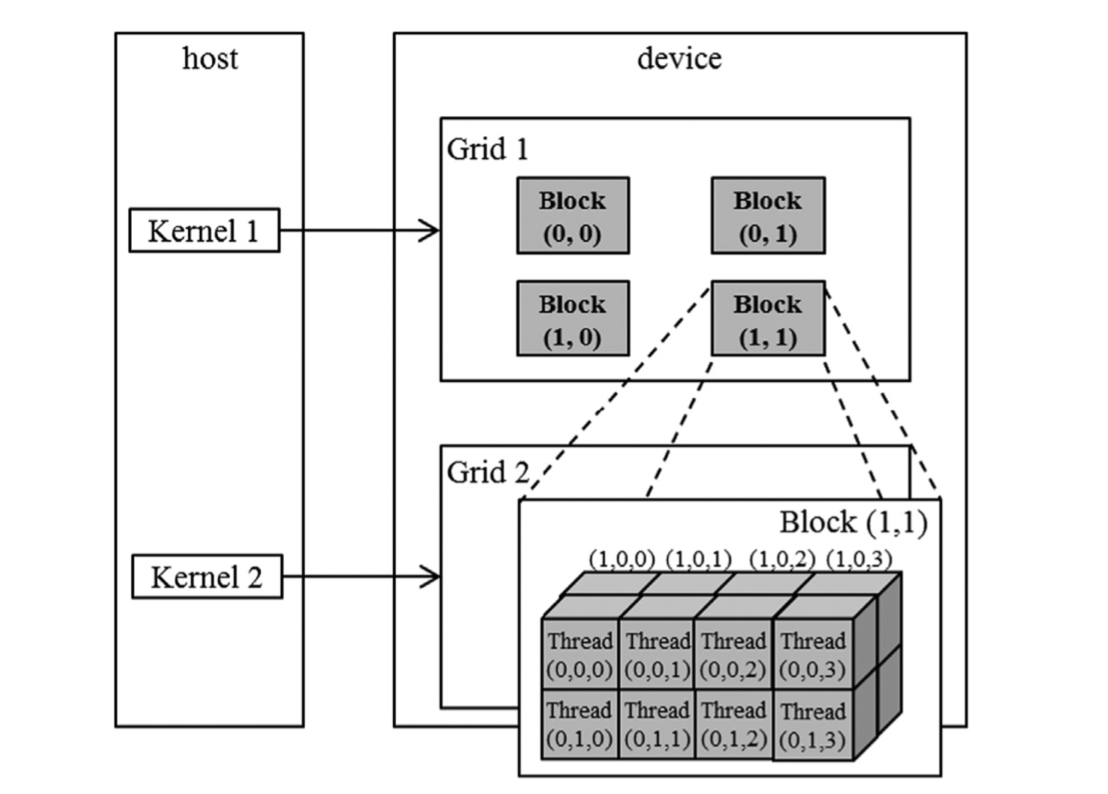
\includegraphics[width=0.9\textwidth]{figs/F3.1.png}
	\caption{\textit{CUDA 网格组织的多维示例。}}
\end{figure}

网格及其块不需要具有相同的维度。 网格可以具有比其块更高的维度,反之亦然。 例如,图 3.1 显示了一个小型玩具网格示例,
其 gridDim 为 (2, 2, 1),blockDim 为 (4, 2, 2)。 可以使用以下主机代码创建这样的网格:

dim3 dimGrid(2, 2, 1);

dim3 dimBlock(4, 2, 2);

KernelFunction<<<dimGrid, dimBlock>>>(...);

图 3.1 中的网格由组织成 $2 \times 2$ 阵列的四个块组成。 每个块都标有(blockIdx.y,blockIdx.x)。 
例如,块 (1,0) 具有 blockIdx.y = 1 和 blockIdx.x = 0。请注意,块和线程标签的顺序是最高维度排在前面。 
此表示法使用的顺序与 C 语句中用于设置配置参数的顺序相反,其中最低维度在前。 
当我们说明在访问多维数据时线程坐标到数据索引的映射时,这种标记块的反向排序效果更好。

每个 threadIdx 还包含三个字段:x 坐标 threadId.x、y 坐标 threadIdx.y 和 z 坐标 threadIdx.z。 
图 3.1 说明了块内线程的组织。 在此示例中,每个块被组织成 $4 \times 2 \times 2$ 个线程数组。 
由于网格内的所有块都具有相同的尺寸,
因此我们仅显示其中之一。 图 3.1 扩展了块 (1,1) 以显示其 16 个线程。 
例如,线程 (1,0,2) 具有 threadIdx.z = 1、threadIdx.y = 0 和 threadIdx.x = 2。
请注意,在本示例中,我们有 4 个块,每个块有 16 个线程,总共有 网格中有 64 个线程。 
我们使用这些小数字是为了保持插图简单。 典型的 CUDA 网格包含数千到数百万个线程。

\subsection{将线程映射到多维数据}
\begin{figure}[H]
	\centering
	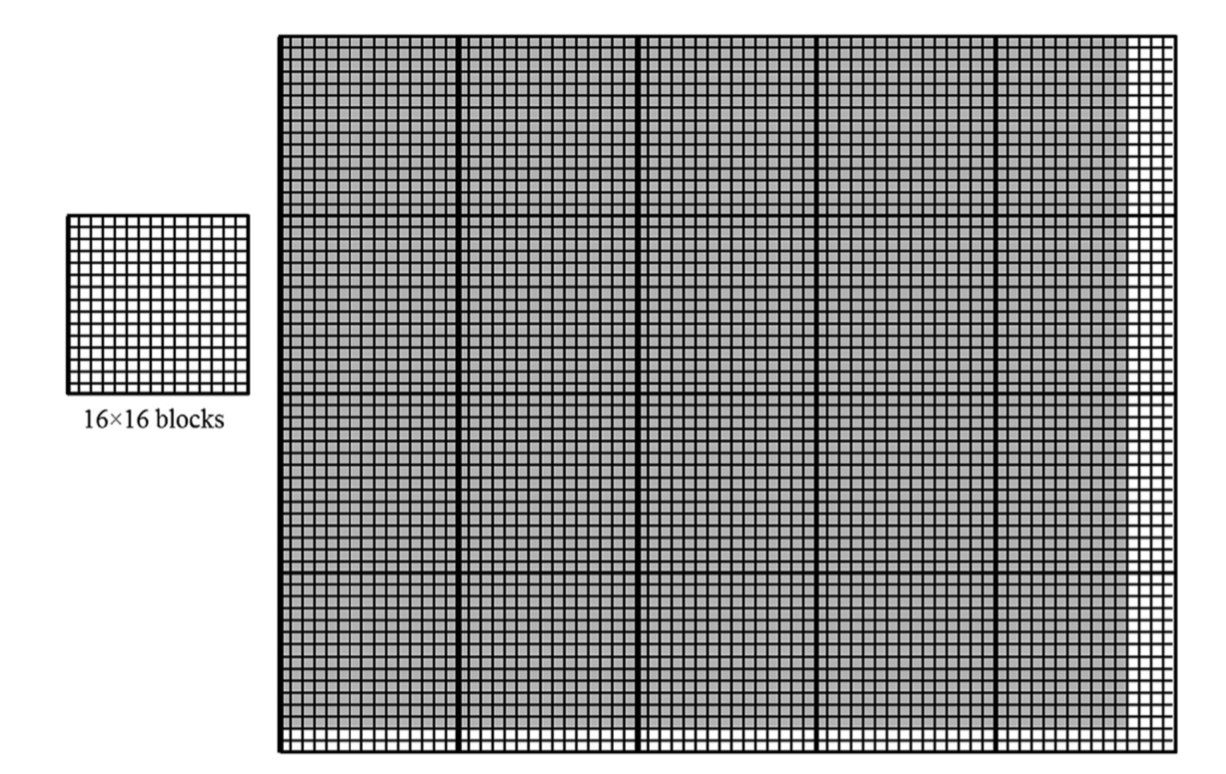
\includegraphics[width=0.9\textwidth]{figs/F3.2.png}
	\caption{\textit{使用2D线程网格处理62*76的图片P。}}
\end{figure}

1D、2D 或 3D 线程组织的选择通常基于数据的性质。 例如,图片是像素的二维阵列。 
使用由 2D 块组成的 2D 网格通常可以方便地处理图片中的像素。 
图3.2示出了用于处理$62 \times 761$F1F
\footnote{我们将按降序引用多维数据的维度:z 维度,然后是 y 维度,依此类推。 
例如,对于垂直或y维度有n个像素、水平或x维度有m个像素的图片,我们将其称为$n \times m$图片。 
这遵循 C 多维数组索引约定。 例如,为了简洁起见,我们可以在文本和图中将 $P[y][x]$ 称为 $P_{y,x}$。 
不幸的是,这种排序与 gridDim 和 blockDim 维度中数据维度的排序顺序相反。 
当我们基于要由其线程处理的多维数组来定义线程网格的维度时,这种差异可能会特别令人困惑。}
图片P(垂直或y方向上62个像素和水平或x方向上76个像素)的这种布置。 
假设我们决定使用 $16 \times 16$ 块,x 方向有 16 个线程,y 方向有 16 个线程。 
我们需要 y 方向上的 4 个块和 x 方向上的 5 个块,这将导致 $4 \times 5 = 20$ 个块,如图 3.2 所示。 
粗线标记了块边界。 阴影区域描绘了覆盖像素的线。 每个线程被分配来处理一个像素,
该像素的 y 和 x 坐标源自其 blockIdx、blockDim 和 threadIdx 变量值:

Vertical(row) row coordinate = blockIdx.y * blockDim.y + threadIdx.y

Horizontal(Column) coordinate = blockIdx.x * blockDim.x + threadIdx.x

例如,块(1,0)的线程(0,0)要处理的Pin元素可以如下标识:
$$
Pin_{blockIdx.y*blockDim.y+threadIdx.y, blockIdx.x*blockDim.x+threadIdx.x} = Pin_{1*16+0,0*16+0} = Pin_{16.0}
$$

请注意,在图 3.2 中,我们在 y 方向上有两个额外的线程,在 x 方向上有四个额外的线程。 
也就是说,我们将生成 $64 \times 80$ 个线程来处理 $62 \times 76$ 个像素。 
这类似于图 2.9 中的 1D 内核 vecAddKernel 使用四个 256 线程块处理 1000 元素向量的情况。 
回想一下,需要图 2.10 中的 if 语句来防止额外的 24 个线程生效。 
同样,我们应该期望图片处理内核函数将具有 if 语句来测试线程的垂直和水平索引是否落在有效的像素范围内。

我们假设主机代码使用整数变量 n 来跟踪 y 方向上的像素数,并使用另一个整数变量 m 来跟踪 x 方向上的像素数。 
我们进一步假设输入的图片数据已经被复制到设备全局内存中并且可以通过指针变量Pin\_d来访问。 
输出图片已分配在设备内存中,可以通过指针变量 Pout\_d 进行访问。 
下面的宿主代码可以调用一个2D内核colorToGrayscaleConversion来处理图片,如下:

dim3 dimGrid(ceil(m/16.0), ceil(n/16.0), 1);

dim3 dimBlock(16, 16, 2);

colorToGrayscaleConversion<<<dimGrid, dimBlock>>>(Pin\_d, Pout\_d, m, n);

在此示例中,为简单起见,我们假设块的尺寸固定为 $16 \times 16$。另一方面,网格的尺寸取决于图片的尺寸。 
为了处理 $1500 \times 2000$(300 万像素)图片,我们将生成 11,750 个块:y 方向 94 个,x 方向 125 个。 
在内核函数中,对 gridDim.x、gridDim.y、blockDim.x 和 blockDim.y 的引用将分别得到 125、94、16 和 16。

在展示内核代码之前,我们首先需要了解 C 语句如何访问动态分配的多维数组的元素。 
理想情况下,我们希望将 Pin\_d 作为 2D 数组进行访问,其中第 j 行和第 i 列的元素可以作为 Pin\_d[j][i] 进行访问。 
然而,开发 CUDA C 所依据的 ANSI C 标准要求在编译时知道 Pin 中的列数,以便将 Pin 作为 2D 数组进行访问。 
不幸的是,对于动态分配的数组,这些信息在编译时是未知的。 
事实上,使用动态分配数组的部分原因是允许这些数组的大小和维度根据运行时的数据大小而变化。 
因此,动态分配的二维数组中的列数信息在编译时是未知的。 
因此,程序员需要显式地将动态分配的 2D 数组线性化或“展平”为当前 CUDA C 中的等效 1D 数组。

实际上,C 中的所有多维数组都是线性化的。 这是由于现代计算机中使用了“平面”内存空间(请参阅“内存空间”侧边栏)。 
对于静态分配的数组,编译器允许程序员使用更高维的索引语法(例如 Pin\_d[j][i])来访问其元素。 
在底层,编译器将它们线性化为等效的一维数组,并将多维索引语法转换为一维偏移量。 
在动态分配数组的情况下,由于编译时缺乏维度信息,当前的 CUDA C 编译器将此类转换的工作留给了程序员。

\begin{remark}[内存空间]
内存空间是现代计算机中处理器如何访问其内存的简化视图。 内存空间通常与每个正在运行的应用程序相关联。 
应用程序要处理的数据和为应用程序执行的指令存储在其存储空间中的位置中。 每个位置通常可以容纳一个字节并具有一个地址。 
需要多个字节的变量(浮点型 4 个字节,双精度型 8 个字节)存储在连续的字节位置中。 
当从内存空间访问数据值时,处理器给出起始地址(起始字节位置的地址)和所需的字节数。

大多数现代计算机至少有 4G 字节大小的位置,其中每个 G 为 1,073,741,824($2^{30}$)。 
所有位置都标有范围从 0 到所使用的最大数字的地址。 由于每个位置只有一个地址,因此我们说内存空间具有“扁平”组织。 
结果,所有多维数组最终都会“展平”为等效的一维数组。 虽然 C 程序员可以使用多维数组语法来访问多维数组的元素,
但编译器会将这些访问转换为指向数组起始元素的基指针,以及根据这些多维索引计算出的一维偏移量。
\end{remark}

至少有两种方法可以使二维数组线性化。 一种是将同一行的所有元素放置到连续的位置。 然后将这些行依次放入内存空间中。 
这种排列称为行优先布局,如图 3.3 所示。 为了提高可读性,我们用 $M_{j,i}$ 来表示 M 中第 j 行第 i 列的元素。 
$M_{j,i}$ 相当于 C 表达式 M[j][i],但可读性稍好一些。 图 3.3 显示了一个示例,
其中 $4 \times 4$ 矩阵 M 被线性化为 16 元素的一维数组,首先是第 0 行的所有元素,然后是第 1 行的 4 个元素,依此类推。 
因此,M 中第 j 行第 i 列的元素的一维等效索引为 $j * 4 + i$。 $j * 4$ 项会跳过 j 行之前的行的所有元素。 
然后,第 i 项在第 j 行的部分中选择正确的元素。 例如,$M_{2,1}$ 的一维索引为 $2 × 4 + 1 = 9$。
如图 3.3 所示,其中 $M_9$ 是与 $M_{2,1}$ 等效的一维索引。 这就是 C 编译器线性化二维数组的方式。

\begin{figure}[H]
	\centering
	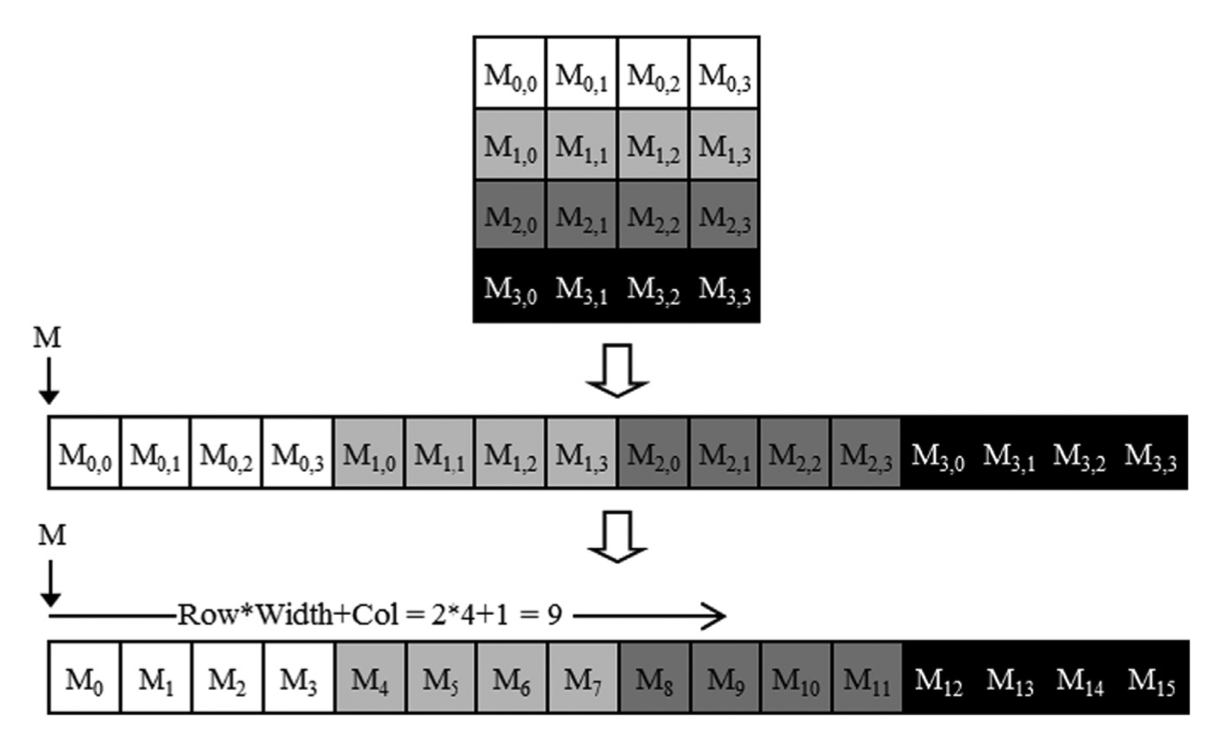
\includegraphics[width=0.9\textwidth]{figs/F3.3.png}
	\caption{\textit{2D C 数组的行优先布局。 结果是一个等效的一维数组,
	通过索引表达式 j × Width+i 访问位于每行 Width 元素数组的第 j 行第 i 列中的元素。}}
\end{figure}

线性化二维数组的另一种方法是将同一列的所有元素放置在连续的位置。 然后将这些列依次放入内存空间中。 
这种排列称为列优先布局,由 FORTRAN 编译器使用。 请注意,二维数组的列优先布局等效于其转置形式的行优先布局。 
我们不会在此花费更多时间,只是要提一下,以前的主要编程经验是使用 FORTRAN 的读者
应该知道 CUDA C 使用行优先布局而不是列优先布局。 
此外,许多设计供 FORTRAN 程序使用的 C 库使用列优先布局来匹配 FORTRAN 编译器布局。 
因此,如果用户从 C 程序调用这些库,这些库的手册页通常会告诉用户转置输入数组。

\begin{figure}[H]
	\centering
	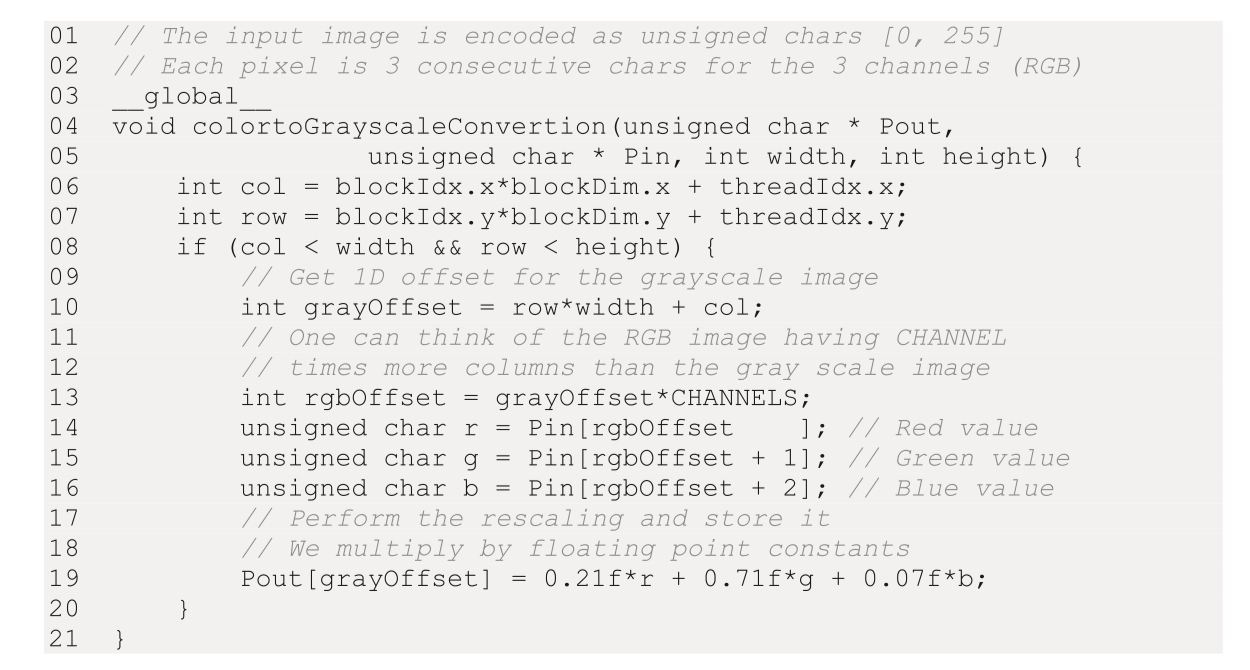
\includegraphics[width=0.9\textwidth]{figs/F3.4.png}
	\caption{\textit{colorToGrayscaleConversion 的源代码,具有 2D 线程映射到数据的功能。}}
\end{figure}

现在我们准备研究colorToGrayscaleConversion的源代码,如图3.4所示。 
内核代码使用以下公式将每个彩色像素转换为其对应的灰度像素:
$$
L = 0.21*r+0.72*g+0.07*b
$$

水平方向总共有 $blockDim.x \times gridDim.x$ 线程。 与 vecAddKernel 示例类似,
以下表达式生成从 0 到 $blockDim.x \times gridDim.x - 1$ 的每个整数值(第 06 行):

col = blockIdx.x*blockDim.x+threadIdx.x

我们知道 $gridDim.x \times blockDim.x$ 大于或等于 width(从主机代码传入的 m 值)。 
我们的线程数至少与水平方向上的像素数一样多。 我们还知道,垂直方向上的线程数至少与像素数一样多。 
因此,只要我们测试并确保只有行和列值都在范围内,即(col < width) \&\& (row < height),
我们就能覆盖图片中的每个像素(第 07 行)。

由于每行都有宽度像素,我们可以为行 row 和列 col 处的像素生成一维索引,即 row × width+col (第 10 行)。 
此 1D 索引 greyOffset 是 Pout 的像素索引,因为输出灰度图像中的每个像素都是 1 个字节(无符号字符)。 
以我们的 $62 \times 76$ 图像为例,块 (1,0) 的线程 (0,0) 计算出 Pout 像素的线性化一维索引,公式如下:
$$
\begin{aligned}
& \text { Pout }_{\text {blockIdx.y*blockDim.y }+ \text { threadIdx.y,blockIdx.x*blockDim.x }+ \text { threadIdx.x }} \\
& =\text { Pout }_{1 * 16+0,0 * 16+0}=\text { Pout }_{16,0}=\operatorname{Pout}[16 * 76+0]=\operatorname{Pout}[1216]
\end{aligned}
$$

至于 Pin,我们需要将灰色像素索引乘以 32F2F
\footnote{我们假设 CHANNELS 是一个值为 3 的常量,并且它的定义在核函数之外。}
(第 13 行),因为每个彩色像素存储为三个元素(r、g、b),
每个元素都是 1 个字节。 生成的 rgbOffset 给出了 Pin 数组中颜色像素的起始位置。 
我们从 Pin 数组的三个连续字节位置读取 r、g 和 b 值(第 14-16 行),执行灰度像素值的计算,
并使用grayOffset 将该值写入 Pout 数组(第 19 行)。 在我们的 $62 \times 76$ 图像示例中,
由块 (1,0) 的线程 (0,0) 处理的 Pin 像素的第一个分量的线性化一维索引可以使用以下公式计算:
$$
\begin{aligned}
& \operatorname{Pin}_{\text {blockIdx.y*blockDim.y }+ \text { threadIdx.y,blockIdx. } x^{*} \text { blockDim.x } x+\text { threadIdx.x }}=\operatorname{Pin}_{1 * 16+0,0 * 16+0} \\
& =\operatorname{Pin}_{16,0}=\operatorname{Pin}\left[16^{*} 76^{*} 3+0\right]=\operatorname{Pin}[3648]
\end{aligned}
$$

正在访问的数据是从字节偏移量 3648 开始的 3 个字节。

\begin{figure}[H]
	\centering
	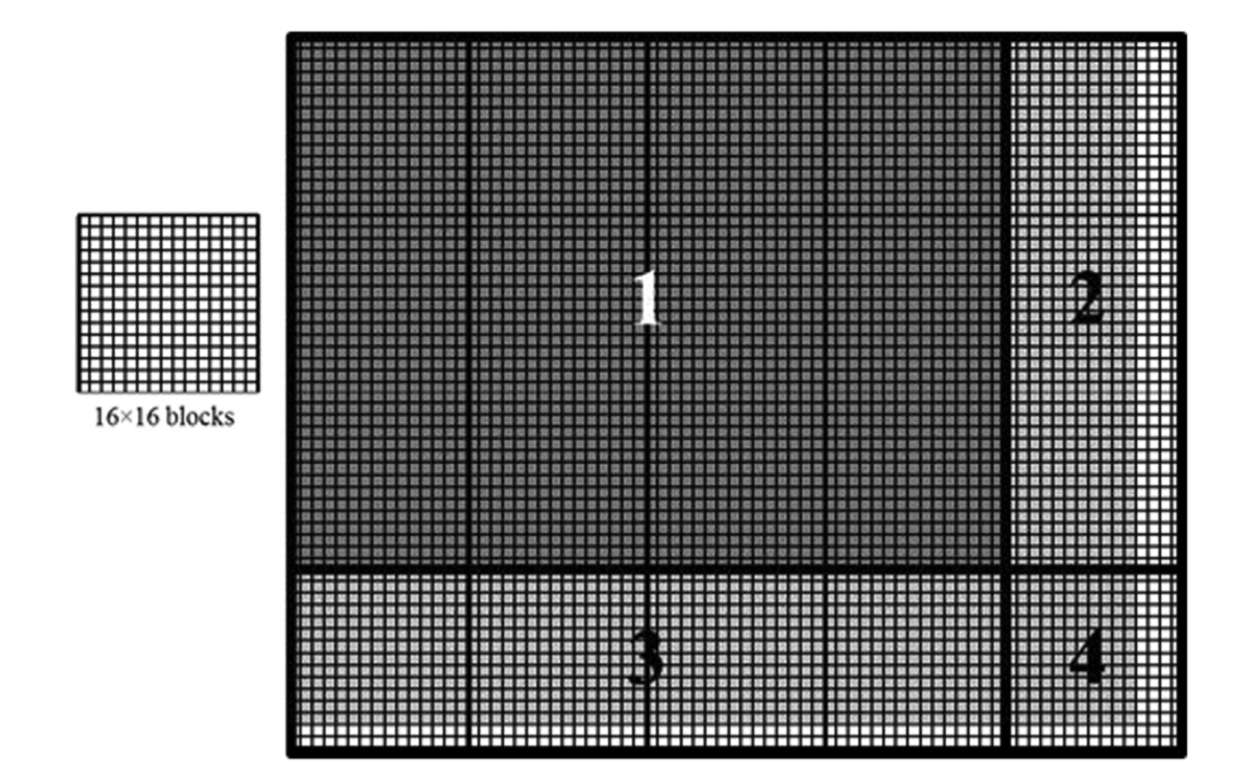
\includegraphics[width=0.9\textwidth]{figs/F3.5.png}
	\caption{\textit{用 16 $\times$ 16 个块覆盖 76 $\times$ 62 的图片。}}
\end{figure}

图 3.5 说明了在处理 $62 \times 76$ 示例时 colorToGrayscaleConversion 的执行情况。 
假设有 $16 \times 16$ 个块,调用 colorToGrayscaleConversion 内核会生成 $64 \times 80$ 个线程。 
网格将有 $4 \times 5 = 20$ 个块:四个在垂直方向,五个在水平方向。 块的执行行为将落入四种不同情况之一,
如图 3.5 中的四个阴影区域所示。

第一个区域在图 3.5 中标记为 1,由属于覆盖图片中大部分像素的 12 个块的线程组成。 这些线程的 col 和 row 值都在范围内; 
所有这些线程都通过了 if 语句测试并处理图片暗阴影区域中的像素。 
也就是说,每个块中的所有 $16 \times 16 = 256$ 个线程将处理像素。

第二个区域,在图 3.5 中标记为 2,包含属于覆盖图片右上像素的中等阴影区域中的三个块的线程。 
虽然这些线程的 row 值始终在范围内,但其中一些线程的 col 值超过了 m 值 76。
这是因为水平方向上的线程数始终是由程序员选择的 blockDim.x 值的倍数(本例中为 16 名)。 
覆盖 76 个像素所需的 16 的最小倍数是 80。因此,每行中的 12 个线程将在范围内找到其 col 值并处理像素。 
每行中剩余的四个线程将发现它们的 col 值超出范围,因此将无法通过 if 语句条件。 这些线程不会处理任何像素。 
总体而言,每个块中的 $16 \times 16 = 256$ 个线程中的 $12 \times 16 = 192$ 个线程将处理像素。

第三个区域,在图 3.5 中标记为 3,占覆盖图片中阴影区域的左下四个块。 
虽然这些线程的 col 值总是在范围内,但其中一些线程的 row 值超过了 n 值 62。
这是因为垂直方向上的线程数始终是由程序员选择的 blockDim.y 值的倍数(本例中为 16 名)。 
16 覆盖 62 的最小倍数是 64。因此,每列中的 14 个线程将在范围内找到其行值并处理像素。 
每列中剩余的两个线程将不会通过 if 语句,并且不会处理任何像素。 
总体而言,256 个线程中的 $16 \times 14 = 224$ 个将处理像素。

第四个区域,在图 3.5 中标记为 4,包含覆盖图片右下浅阴影区域的线。 
与区域 2 一样,前 14 行中每一行中的 4 个线程都会发现它们的 col 值超出范围。 
与区域 3 一样,该块的整个底部两行将发现其行值超出范围。 
总体而言,$16 \times 16 = 256$ 个线程中只有 $14 \times 12 = 168$ 个线程会处理像素。

通过在线性化数组时包含另一个维度,我们可以轻松地将 2D 数组的讨论扩展到 3D 数组。 
这是通过将数组的每个“平面”依次放入地址空间来完成的。 假设程序员使用变量 m 和 n 分别跟踪 3D 数组中的列数和行数。 
程序员在调用内核时还需要确定 blockDim.z 和 gridDim.z 的值。 在内核中,数组索引将涉及另一个全局索引:

int plane = blockIdx.z * blockDim.z + threadIdx.z

对 3D 数组 P 的线性化访问将采用 $P[plane * m * n +row * m+col]$ 的形式。 
处理 3D P 数组的内核需要检查所有三个全局索引(plane、row 和 col)是否落在数组的有效范围内。 
CUDA 内核中 3D 数组的使用将在第 8 章 Stencil 中对模板模式进行进一步研究。

\subsection{图像模糊:一个更复杂的核函数}
我们研究了 vecAddkernel 和 colorToGrayscaleConversion,其中每个线程仅对一个数组元素执行少量算术运算
这些内核很好地满足了它们的目的:说明基本的 CUDA C 程序结构和数据并行执行概念。 
此时,读者应该问一个显而易见的问题:CUDA C 程序中的所有线程是否仅彼此独立地执行如此简单且琐碎的操作? 答案是不。 
在实际的CUDA C程序中,线程经常对其数据执行复杂的操作,并且需要相互协作。 
在接下来的几章中,我们将研究展示这些特征的日益复杂的示例。 我们将从图像模糊函数开始。

\begin{figure}[H]
	\centering
	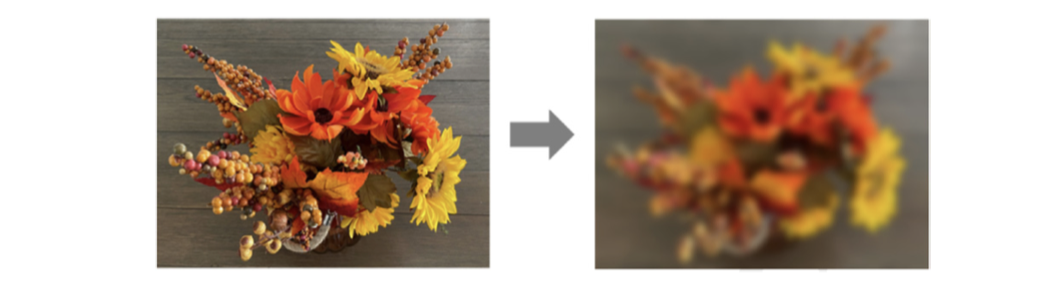
\includegraphics[width=0.9\textwidth]{figs/F3.6.png}
	\caption{\textit{原始图像(左)和模糊版本(右)。}}
\end{figure}

图像模糊可以消除像素值的突然变化,同时保留对于识别图像关键特征至关重要的边缘。 图 3.6 说明了图像模糊的效果。 
简单地说,我们使图像变得模糊。 对于人眼来说,模糊的图像往往会掩盖细节并呈现“大局”印象,或者图片中的主要主题对象。 
在计算机图像处理算法中,图像模糊的常见用例是通过使用干净的周围像素值校正有问题的像素值来减少图像中噪声和颗粒渲染效果的影响。 
在计算机视觉中,图像模糊可用于允许边缘检测和对象识别算法专注于主题对象,而不是被大量细粒度对象所困扰。 
在显示器中,图像模糊有时用于通过模糊图像的其余部分来突出显示图像的特定部分。

从数学上讲,图像模糊函数将输出图像像素的值计算为包含输入图像中像素的像素块的加权和。 
正如我们将在第 7 章“卷积”中了解到的那样,此类加权和的计算属于卷积模式。 
在本章中,我们将使用一种简化的方法,对目标像素周围(包括目标像素)的 $N \times N$ 像素块取简单平均值。 
为了保持算法简单,我们不会根据与目标像素的距离对任何像素的值进行权重。 
实际上,放置这样的权重在卷积模糊方法中很常见,例如高斯模糊。

\begin{figure}[H]
	\centering
	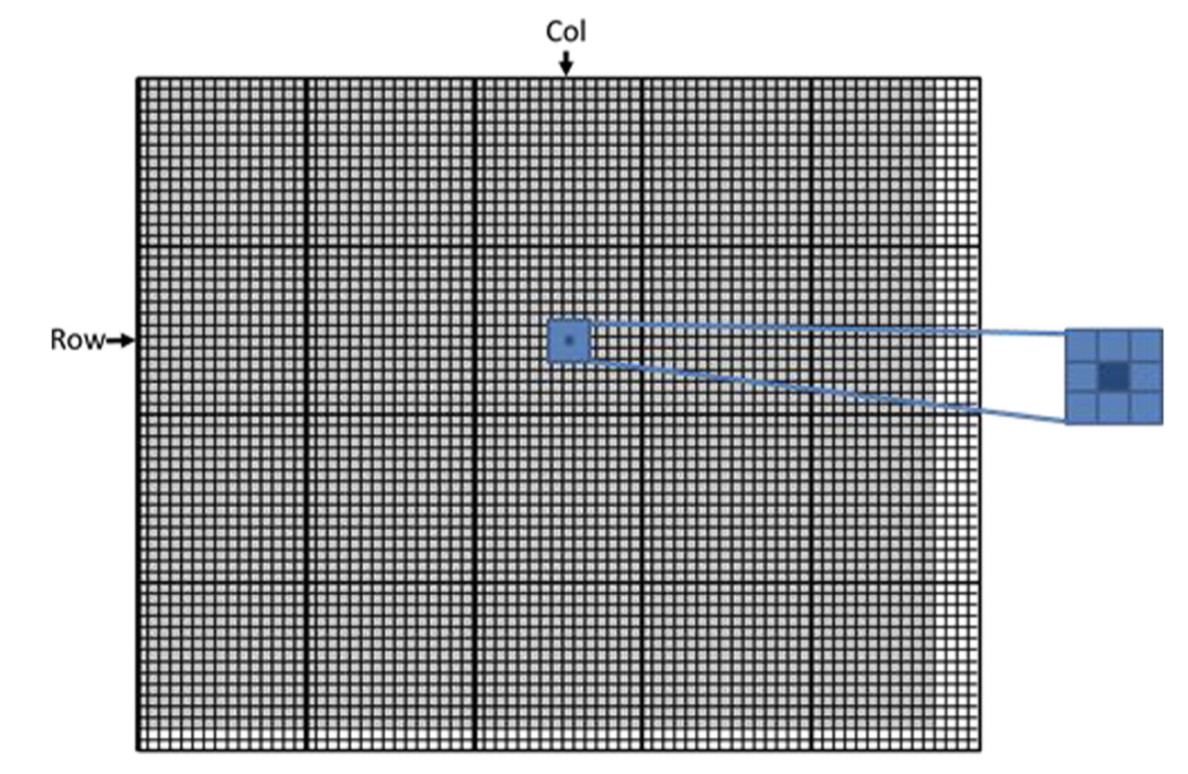
\includegraphics[width=0.9\textwidth]{figs/F3.7.png}
	\caption{\textit{每个输出像素是输入图像中周围像素块及其自身的平均值。}}
\end{figure}

图 3.7 显示了使用 $3 \times 3$ 补丁进行图像模糊的示例。 当计算(行,列)位置处的输出像素值时,
我们看到补丁以位于(行,列)位置的输入像素为中心。 $3 \times 3$ 补丁跨越三行(row-1、row、row+1)
和三列(col-1、col、col+1)。 例如,计算(25, 50)处输出像素的9个像素的坐标
分别为(24, 49)、(24, 50)、(24, 51)、(25, 49)、(25, 50) 、(25, 51)、(26, 49)、(26, 50) 和(26, 51)。

\begin{figure}[H]
	\centering
	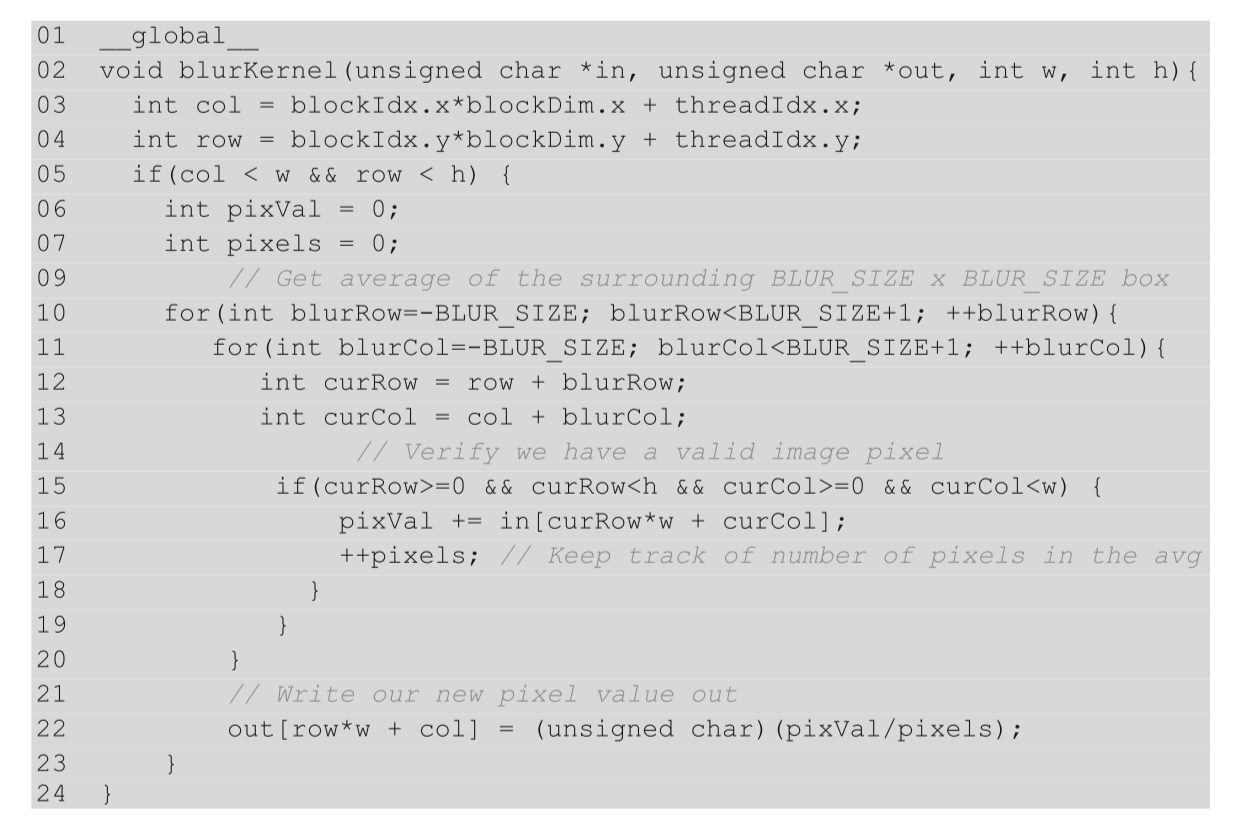
\includegraphics[width=0.9\textwidth]{figs/F3.8.png}
	\caption{\textit{图像模糊内核。}}
\end{figure}

图 3.8 显示了图像模糊内核。 与 colorToGrayscaleConversion 中使用的策略类似,我们使用每个线程来计算输出像素。 
也就是说,线程到输出数据的映射保持不变。 因此,在内核的开头,我们看到了熟悉的列索引和行索引的计算(第 03-04 行)。 
我们还看到了熟悉的 if 语句,它根据图像的高度和宽度验证 col 和 row 是否在有效范围内(第 05 行)。 
只有列索引和行索引都在值范围内的线程才允许参与执行。

如图 3.7 所示,col 和 row 值还给出了用于计算线程输出像素的输入像素块的中心像素位置。 
图 3.8(第 10-11 行)中的嵌套 for 循环迭代块中的所有像素。 我们假设程序有一个已定义的常量 BLUR\_SIZE。 
BLUR\_SIZE 的值设置为使得 BLUR\_SIZE 给出面片每侧(半径)上的像素数,2 × BLUR\_SIZE+1 给出面片一维上的像素总数。 
例如,对于 3 x 3 补丁,BLUR\_SIZE 设置为 1,而对于 7 x 7 补丁,BLUR\_SIZE 设置为 3。
外循环迭代补丁的行。 对于每一行,内部循环都会迭代补丁的列。

在我们的 3 x 3 补丁示例中,BLUR\_SIZE 为 1。对于计算输出像素 (25, 50) 的线程,在外循环的第一次迭代期间,
curRow 变量为 row-BLUR\_SIZE$ = (25 - 1) = 24$ 因此,在外循环的第一次迭代期间,内循环迭代第 24 行中的块像素。
内循环使用 curCol 变量从列 col-BLUR\_SIZE$ = 50 - 1 = 49$ 迭代到 col+BLUR\_SIZE$ = 51$。 
因此,在外循环的第一次迭代中处理的像素是 (24, 49)、(24, 50) 和 (24, 51)。 
读者应该验证在外循环的第二次迭代中,内循环迭代像素 (25, 49)、(25, 50) 和 (25, 51)。 
最后,在外循环的第三次迭代中,内循环迭代像素 (26, 49)、(26, 50) 和 (26, 51)。

第 16 行使用 curRow 和 curCol 的线性化索引来访问当前迭代中访问的输入像素的值。 
它将像素值累积到运行总和变量 pixVal 中。 第 17 行记录了这样一个事实:通过增加像素变量,
又将一个像素值添加到运行总和中。 处理完 patch 中的所有像素后,
第 22 行通过将 pixVal 值除以像素值来计算 patch 中像素的平均值。 它使用行和列的线性化索引将结果写入其输出像素。

\begin{figure}[H]
	\centering
	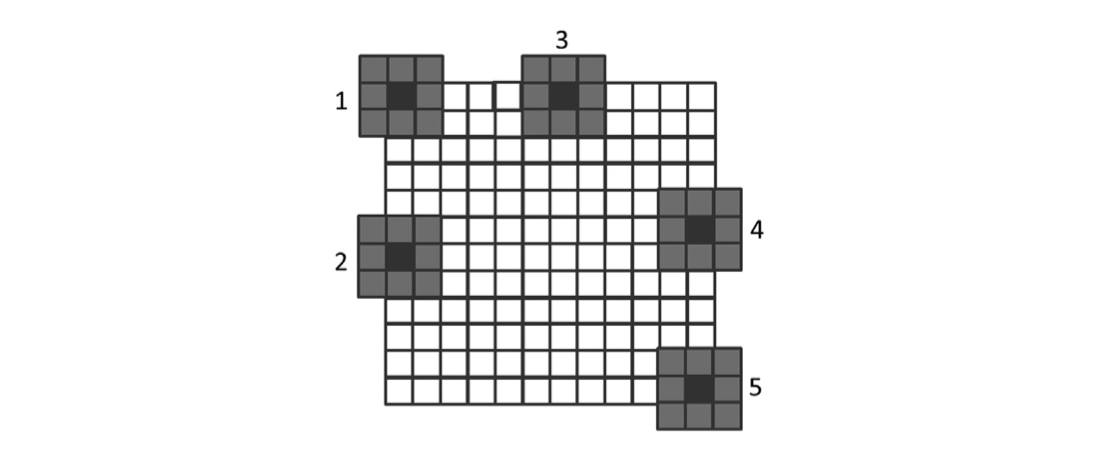
\includegraphics[width=0.9\textwidth]{figs/F3.9.png}
	\caption{\textit{处理图像边缘附近像素的边界条件。}}
\end{figure}

第 15 行包含一个条件语句,用于保护第 16 行和第 17 行的执行。例如,在计算图像边缘附近的输出像素时,
补丁可能会超出输入图像的有效范围。 这在图 3.9 中进行了说明,假设有 3 x 3 个补丁。 在情况 1 中,左上角的像素变得模糊。 
输入图像中不存在预期补丁中的九个像素中的五个。 在这种情况下,输出像素的行和列值分别为0和0。 
在嵌套循环的执行过程中,九次迭代的 curRow 和 curCol 值
为 (21, 2 1), (21,0), (21,1), (0, 2 1), (0,0), (0,1)、(1, 2 1)、(1,0) 和 (1,1)。 
请注意,对于图像外部的 5 个像素,至少有一个值小于 0。 if 语句的 curRow < 0 和 curCol < 0 条件捕获这些值
并跳过第 16 行和第 17 行的执行。 结果,只有四个有效像素的值被累加到运行和变量中。 
像素值也仅正确增加四次,以便可以在第 22 行正确计算平均值。

读者应该研究图3.9中的其他情况并分析blurKernel中嵌套循环的执行行为。 
请注意,大多数线程将在输入图像中找到其分配的 3 x 3 块中的所有像素。 他们将累积所有九个像素。 
然而,对于四个角上的像素,负责的线程只会累积四个像素。 对于四个边缘上的其他像素,负责的线程将累积六个像素。 
这些变化使得需要跟踪与可变像素一起累积的实际像素数。

\subsection{矩阵乘法}
矩阵-矩阵乘法,或简称矩阵乘法,是基本线性代数子程序标准的重要组成部分(请参阅“线性代数函数”边栏)。 
它是许多线性代数求解器的基础,例如 LU 分解。 这也是使用卷积神经网络进行深度学习的重要计算,
这将在第 16 章“深度学习”中详细讨论。

\begin{remark}[线性代数函数]
	线性代数运算广泛应用于科学和工程应用中。 在基本线性代数子程序 (BLAS)(执行基本代数运算的发布库的事实上的标准)中,
	存在三个级别的线性代数函数。 随着级别的提高,函数执行的操作数量也会增加。 
	1 级函数执行 $\bm y = \alpha \bm x+\bm y$ 形式的向量运算,其中 $\bm x$ 和 $\bm $y 是向量,$\alpha$ 是标量。 
	我们的向量加法示例是具有 $\alpha = 1$ 的 1 级函数的特例。
	2 级函数执行 $y = \alpha \bm A\bm x+\beta \bm y$ 形式的矩阵向量运算,
	其中 $\bm A$ 是矩阵,$\bm x$ 和 $\bm y$ 是向量,
	$\alpha$ 和 $\beta$ 是 标量。 我们将研究稀疏线性代数中的 2 级函数的一种形式。 
	3 级函数以 $C = \alpha \bm A\bm B + \beta \bm C$ 的形式执行矩阵-矩阵运算,
	其中 $\bm A$、$\bm B$ 和 $\bm C$ 是矩阵,$\alpha$ 和 $\beta$ 是标量。 
	我们的矩阵-矩阵乘法示例是 3 级函数的特例,其中 $\alpha = 1$ 和 $\beta = 0$。这些 BLAS 函数很重要,
	因为它们用作高级代数函数的基本构建块,例如线性系统求解器和 特征值分析。 
	正如我们稍后将讨论的,BLAS 函数的不同实现的性能在顺序计算机和并行计算机中可能存在数量级的差异。
\end{remark}

$\mathrm{I} \times \mathrm{j}$($\mathrm{i}$ 行乘以 $\mathrm{j}$ 列)矩阵 $M$ 
和 $\mathrm{j} \times \mathrm{k}$ 矩阵 $\mathrm{N}$ 之间的矩阵乘法
生成 $\mathrm{I} \times \mathrm{k}$ 矩阵 $\mathrm{P}$。 
当进行矩阵乘法时,输出矩阵$P$的每个元素都是行$M$和列$\mathrm{N}$的内积。 
我们将继续使用约定,其中 $\mathrm{P}_{\text {row, col }}$ 是垂直方向上第 rowth 位置和水平方向上第 colth 位置的元素。 
如图3.10所示,$\mathrm{P}_{\text {row,col }}$($\mathrm{P}$中的小方块)
是由第row行形成的向量的内积 $M$(在 $M$ 中显示为水平条带)和由 $N$ 的 colth 列形成的向量(在 N 中显示为垂直条带)。 
两个向量的内积(有时称为点积)是各个向量元素的乘积之和。
$$
\mathrm{P}_{\text {row }, \mathrm{col}}=\sum \mathrm{M}_{\text {row }, \mathrm{k}}{ }^{*} \mathrm{~N}_{\mathrm{k}, \mathrm{col}} \quad \text { for } \mathrm{k}=0,1, \ldots \text { Width }-1
$$

\begin{figure}[H]
	\centering
	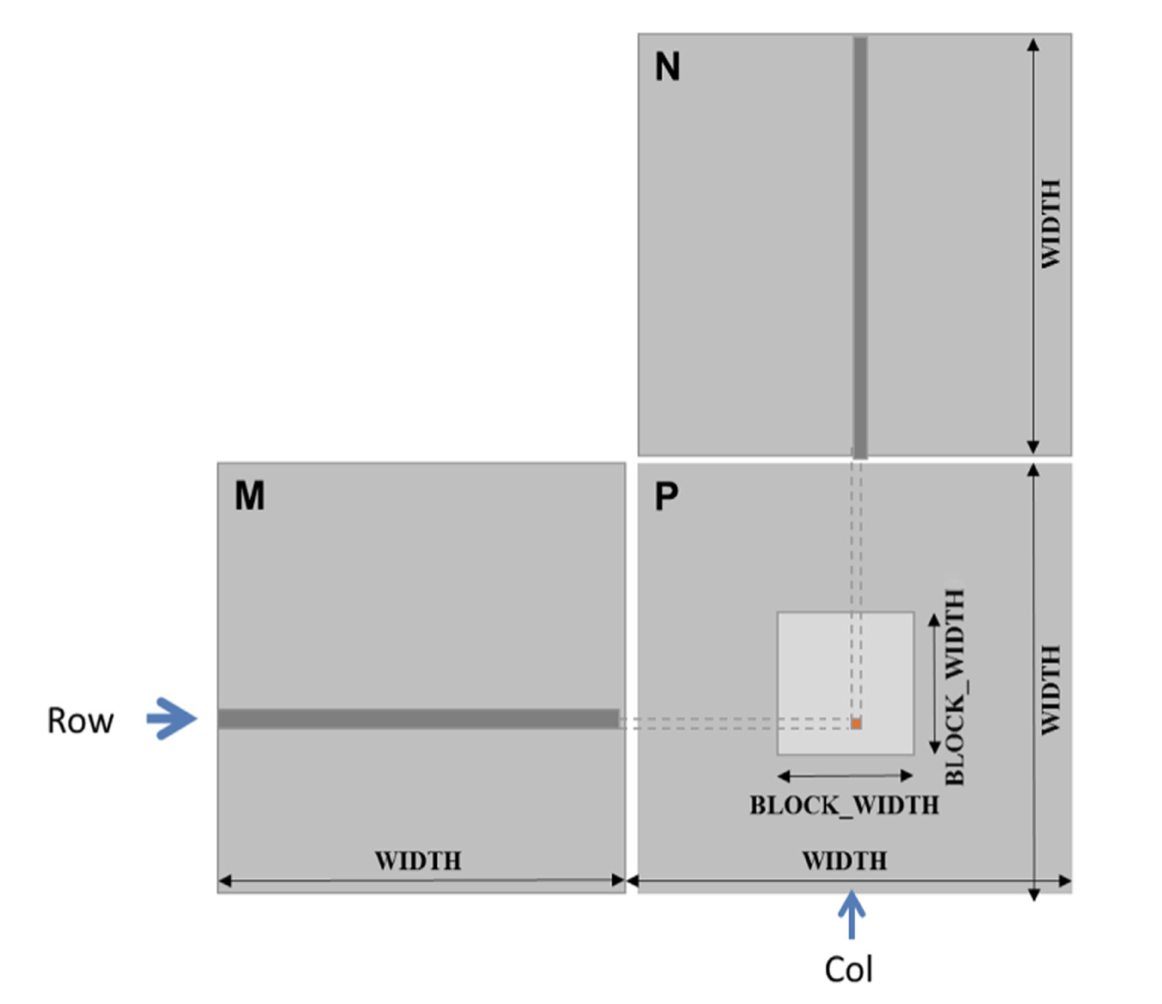
\includegraphics[width=0.9\textwidth]{figs/F3.10.png}
	\caption{\textit{通过平铺 P 使用多个块进行矩阵乘法。}}
\end{figure}

例如,在图 3.10 中,假设行 $=1$ 且 $\mathrm{col}=5$,
$$
\mathrm{P}_{1,5}=\mathrm{M}_{1,0}{ }^{*} \mathrm{~N}_{0,5}+\mathrm{M}_{1,1}{ }^{*} \mathrm{~N}_{1,5}+\mathrm{M}_{1,2}{ }^{*} \mathrm{~N}_{2,5}+\ldots .+\mathrm{M}_{1, \text { Width }-1}{ }^{*} \mathrm{~N}_{\text {Width-1,5}}
$$

要使用 CUDA 实现矩阵乘法,我们可以使用与 colorToGrayscaleConversion 相同的方法
将网格中的线程映射到输出矩阵 P 的元素。 即每个线程负责计算一个P元素。 
每个线程要计算的 P 元素的行索引和列索引与之前相同:
$$
\text { row }=\text { blockIdx } \cdot y^{\star} \text { blockDim.y }+ \text { threadIdx } \cdot y
$$

和
$$
\operatorname{col}=\text { blockIdx.x*blockDim.x }+ \text { threadIdx.x }
$$

\begin{figure}[H]
	\centering
	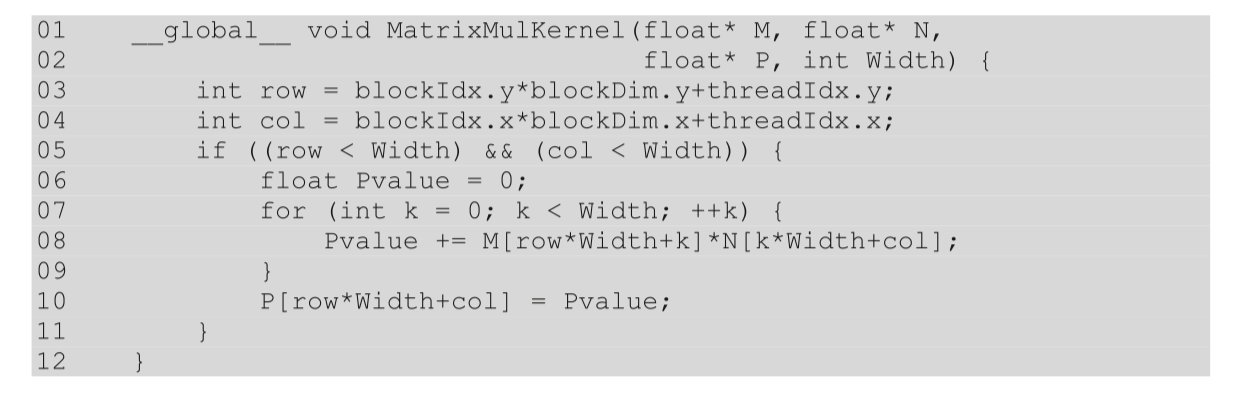
\includegraphics[width=0.9\textwidth]{figs/F3.11.png}
	\caption{\textit{使用一个线程计算一个 P 元素的矩阵乘法内核。}}
\end{figure}

通过这种一对一映射,行和列线程索引也是其输出元素的行和列索引。 图 3.11 显示了基于线程到数据映射的内核源代码。 
读者应该立即看到熟悉的计算 row 和 col 的模式(第 03-04 行)以及测试 row 和 col 是否都在范围内的 if 语句(第 05 行)。 
这些语句与 colorToGrayscaleConversion 中的对应语句几乎相同。 
唯一显着的区别是,我们做出了一个简化的假设:matrixMulKernel 只需要处理方阵,因此我们将宽度和高度都替换为 Width。 
这种线程到数据的映射有效地将 P 划分为图块,其中一个图块在图 3.10 中显示为浅色方块。 每个块负责计算这些图块之一。

现在我们将注意力转向每个线程所做的工作。 回想一下,$P_{row,col}$ 计算为 M 的第 rowth 行和 N 的 colth 列的内积。
在图 3.11 中,我们使用 for 循环来执行此内积运算。 在进入循环之前,我们将局部变量 Pvalue 初始化为 0(第 06 行)。 
循环的每次迭代都会访问 M 的第 rowth 行中的一个元素和 N 的 colth 列中的一个元素,
将两个元素相乘,并将乘积累加到 Pvalue 中(第 08 行)。

让我们首先关注在 for 循环中访问 M 元素。 使用行主序将 M 线性化为等效的一维数组。 
即M的行从第0行开始依次放置在内存空间中。 因此,第 1 行的起始元素是 M[1 $\times$ Width],因为我们需要考虑第 0 行的所有元素。
一般来说,第 1 行的起始元素是 M[row $\times$ Width]。 由于一行的所有元素都放置在连续的位置,
因此第 rowth 行的第 k 个元素位于 M[row $\times$ Width+k]。 这个线性化数组偏移量就是我们在图 3.11(第 08 行)中使用的。

现在我们将注意力转向访问N。如图3.11所示,colth列的起始元素是第0行的colth元素,即N[col]。 
访问 colth 列中的下一个元素需要跳过整行。 这是因为同一列的下一个元素与下一行中的相同元素。 
因此,colth 列的第 k 个元素是 N[k $\times$ Width+col](第 08 行)。

执行退出 for 循环后,所有线程的 Pvalue 变量中都有其 P 元素值。 
然后,每个线程使用 1D 等效索引表达式 row $\times$ Width+col 写入其 P 元素(第 10 行)。 
同样,此索引模式类似于 colorToGrayscaleConversion 内核中使用的索引模式。

\begin{figure}[H]
	\centering
	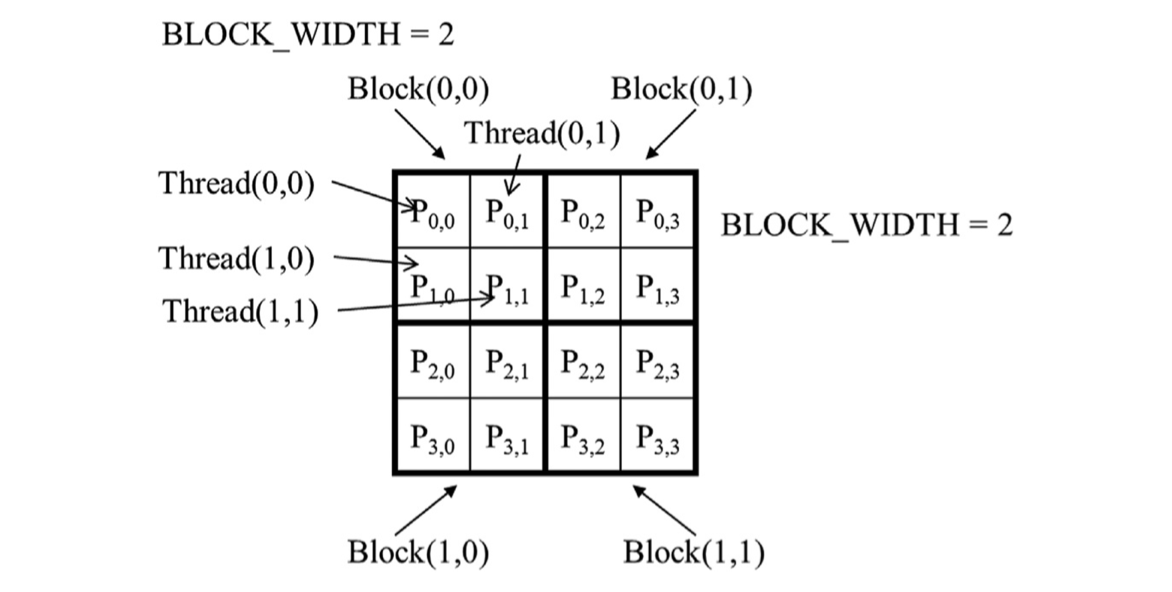
\includegraphics[width=0.9\textwidth]{figs/F3.12.png}
	\caption{\textit{matrixMulKernel 的一个小型执行示例。}}
\end{figure}

我们现在用一个小例子来说明矩阵乘法内核的执行。 图 3.12 显示了 BLOCK\_WIDTH = 2 的 $4\times 4$P。
虽然如此小的矩阵和块大小不太现实,但它们允许我们将整个示例放入一张图片中。 P矩阵被分为4个tile,
每个块计算一个tile。 我们通过创建由 $2\times 2$ 个线程数组组成的块来实现这一点,每个线程计算一个 P 元素。 
在该示例中,块 (0,0) 的线程 (0,0) 计算 $P_{0,0}$ ,而块 (1,0) 的线程 (0,0) 计算 $P_{2,0}$。

\begin{figure}[H]
	\centering
	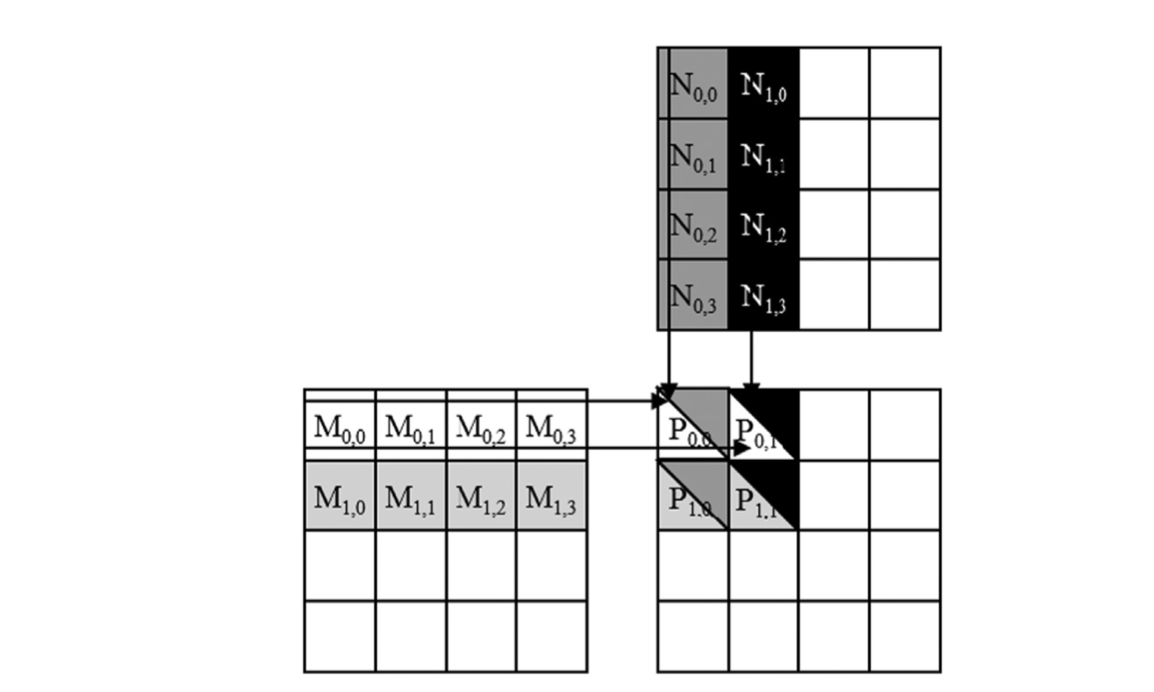
\includegraphics[width=0.9\textwidth]{figs/F3.13.png}
	\caption{\textit{一个线程块的矩阵乘法运算。}}
\end{figure}

matrixMulKernel 中的 row 和 col 索引标识要由线程计算的 P 元素。 行索引还标识 M 的行,
列索引标识 N 的列作为线程的输入值。 图 3.13 说明了每个线程块中的乘法运算。 
对于小矩阵乘法示例,块 (0,0) 中的线程产生四个点积。 块(0,0)中线程(1,0)的行索引和列索引分别为$0*0 + 1 = 1$
和$0 * 0 + 0 = 0$。 因此,线程映射到 $P_{1,0}$ 并计算 M 的第 1 行和 N 的第 0 列的点积。

让我们看一下图 3.11 中线程 (0,0) 在块 (0,0) 中的 for 循环的执行情况。 
在迭代 $0(k = 0)$ 期间,row $\times$ Width + k = 0 * 4 + 0 = 0 和 k $\times$ Width + col = 0 * 4 + 0 = 0。
因此,访问的输入元素是 M[0] 和 N [0],它们是 1D 等价的 $M_{0,0}$ 和 $N_{0,0}$ 。 
请注意,这些确实是 M 的第 0 行和 N 的第 0 列的第 0 个元素。在迭代 $1(k = 1)$ 期间,
row $\times$ Width + k = 0 * 4 + 1 = 1 和 k $\times$ Width + col = 1 $\times$ 4 + 0 = 4。
因此 我们正在访问 M[1] 和 N[4],
它们是 $M_{0,1}$ 和 $N_{1,0}$ 的一维等价物。 这些是 M 的第 0 行和 N 的第 0 列的第一个元素。
在迭代 $2(k = 2)$ 期间, row $\times$ Width + k = 0 $\times$ 4 + 2 = 2 
和 k $\times$ Width + col = 2 $\times$ 4 + 0 = 8,
结果为 M [2]和N[8]。 因此,访问的元素是 $M_{0,2}$ 和 $N_{2,0}$ 的一维等效项。
最后,在迭代 3 (k = 3) 期间,row $\times$ Width + k = 0 $\times$ 4 + 3 = 3 
和 k $\times$ Width + col = 3 $\times$ 4 + 0 = 12,结果是 M[3] 和 N[12],即 M 的一维等价物 $M_{0,3}$ 和 $N_{3,0}$。 
现在我们已经验证了 for 循环在块 (0,0) 中对线程 (0,0) 执行 M 第 0 行和 N 第 0 列之间的内积。 
循环结束后,线程写入P[行$\times$ 宽度+列],即P[0]。 这是 $P_{0,0}$ 的一维等效项,
因此块 (0,0) 中的线程 (0,0) 成功计算了 M 的第 0 行和 N 的第 0 列之间的内积,并将结果存放在 $P_{0,0}$ 中。

我们将把它作为一个练习,让读者手动执行和验证块 (0,0) 或其他块中其他线程的 for 循环。

由于网格的大小受到每个网格的最大块数和每个块的线程数的限制,
因此,matrixMulKernel 可以处理的最大输出矩阵 P 的大小也将受到这些约束的限制。 
在要计算大于此限制的输出矩阵的情况下,可以将输出矩阵划分为大小可以被网格覆盖的子矩阵,
并使用主机代码为每个子矩阵启动不同的网格。 或者,我们可以更改内核代码,以便每个线程计算更多的 P 元素。 
我们将在本书后面探讨这两种选择。

\subsection{总结}
CUDA 网格和块是多维的,最多三个维度。 网格和块的多维性对于组织要映射到多维数据的线程很有用。 
内核执行配置参数定义网格及其块的维度。 blockIdx 和 threadIdx 中的唯一坐标允许网格线程识别自身及其数据域。 
程序员有责任在内核函数中使用这些变量,以便线程可以正确识别要处理的数据部分。 
当访问多维数据时,程序员通常必须将多维索引线性化为一维偏移量。 
原因是 C 中动态分配的多维数组通常以行优先顺序存储为一维数组。 
我们使用日益复杂的示例来让读者熟悉使用多维网格处理多维数组的机制。 这些技能将是理解并行模式及其相关优化技术的基础。